\documentclass[10pt]{beamer}

\beamertemplatenavigationsymbolsempty

\usepackage{multicol}
\usepackage[czech]{babel}
\usepackage[utf8]{inputenc}
\usepackage[T1]{fontenc}
\usepackage{booktabs}
\usepackage[scale=2]{ccicons}

\usepackage{diagbox}
\newcommand{\labelkm}{\scriptsize \diagbox[width=13pt,height=15pt]
        {\raisebox{-0pt}{k}}{ \raisebox{1pt}{m} } }


\usepackage{tikz}

\usepackage{gnuplottex}

\usepackage{booktabs,longtable}%
\usepackage{colortbl}%
\newcommand{\evenrowcolor}{\rowcolor[gray]{0.925}}

\title{
Practical Exhaustive Generation of Small
Multiway Cuts in Sparse Graphs
}
\subtitle{}
\date{}
\author{Petr Hliněný and Ondřej Slámečka}
\institute{Faculty of Informatics, Masaryk University, Brno}

\begin{document}

\maketitle

\begin{frame}
	\frametitle{Accidents, disasters and roads}

	Going from A to B when suddenly\ldots
\end{frame}

\begin{frame}
	\frametitle{Accidents, disasters and roads}
	\noindent\makebox[\textwidth]{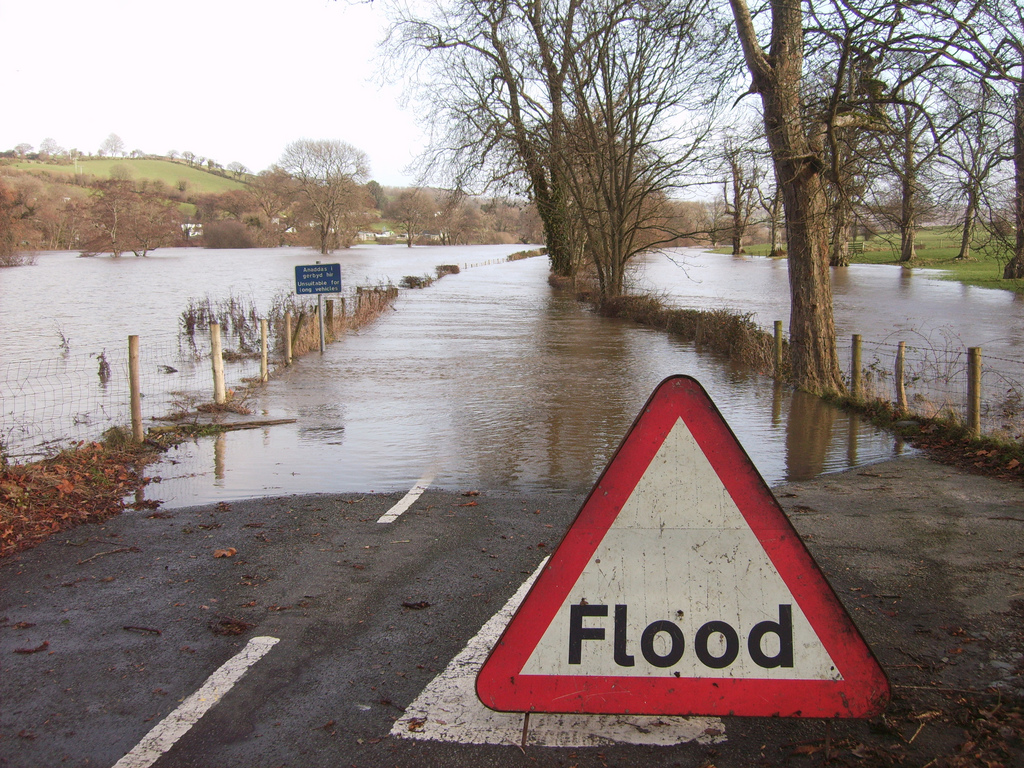
\includegraphics[width=\paperwidth]{images/flood.jpg}}
\end{frame}

\begin{frame}
	\frametitle{Accidents, disasters and roads}
	\noindent\makebox[\textwidth]{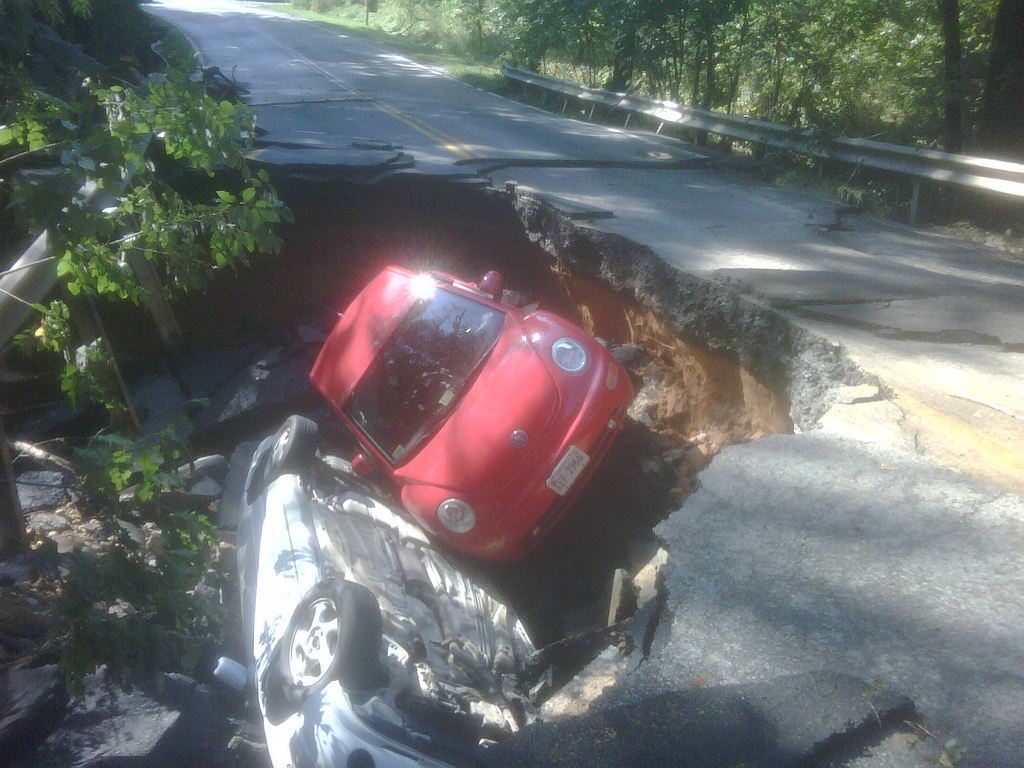
\includegraphics[width=\paperwidth]{images/road_wash.jpg}}
\end{frame}

\begin{frame}
	\frametitle{Accidents, disasters and roads}
	\noindent\makebox[\textwidth]{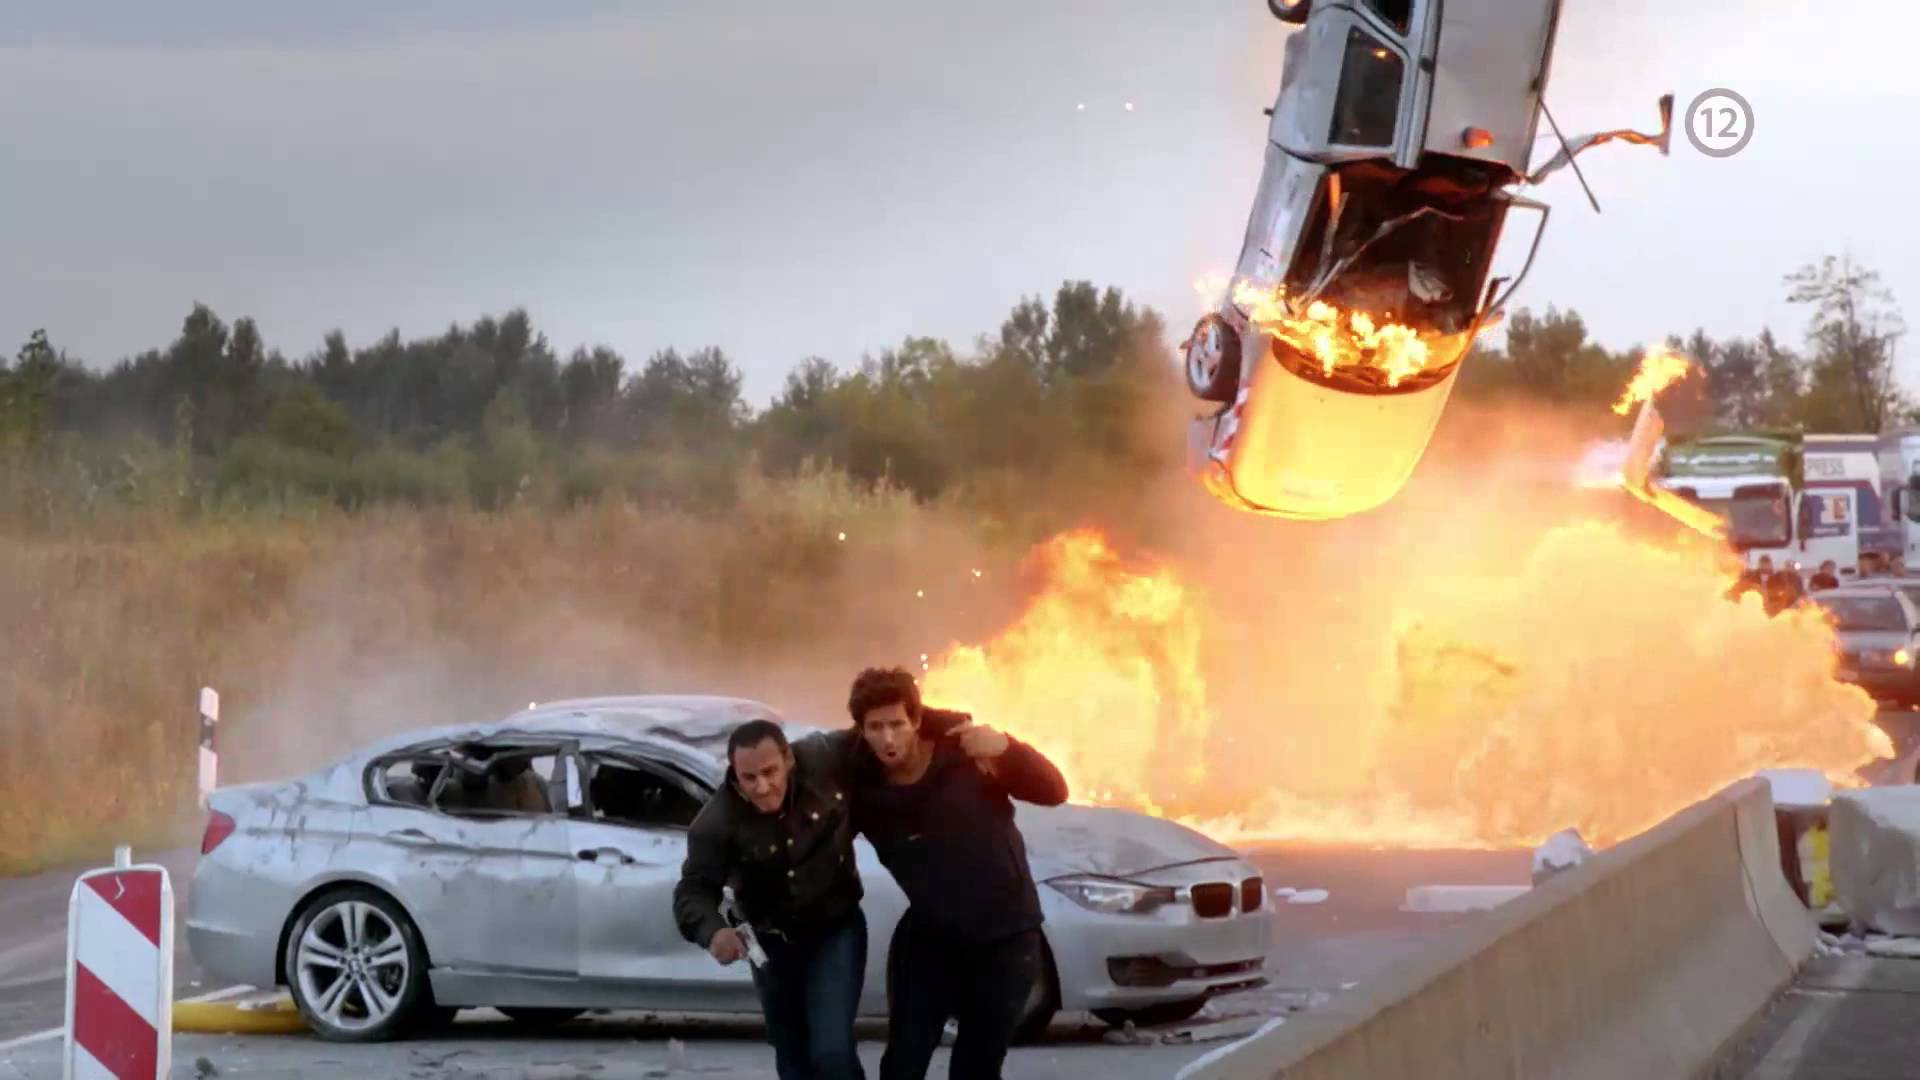
\includegraphics[width=\paperwidth]{images/kobra_11.jpg}}
\end{frame}

\begin{frame}
	\frametitle{Accidents, disasters and roads}

	Our way to B is cut.

	\bigskip

	Can this happen in situations other than travelling?
\end{frame}

\begin{frame}
	\frametitle{Networks}
	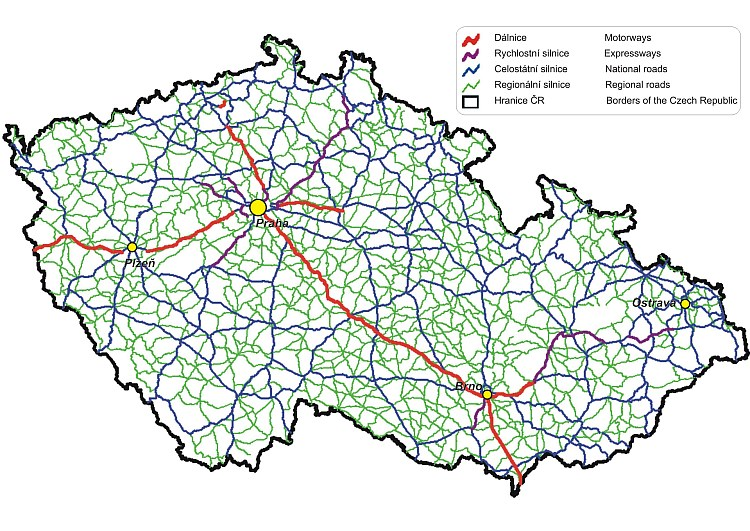
\includegraphics[width=\textwidth]{images/road_network.jpg}

	Not just roads. Also internet, electrical grid, bridges of Königsberg,\ldots
\end{frame}


\begin{frame}[fragile]
	\frametitle{The problem}


	For a given (sparse) graph $G = (V, E)$ find all the minimal (wrt.
	inclusion) sets $X \subseteq E$ such that, $G \setminus X$ has $k$
	connected components. \\

	\bigskip

	\bigskip
	\textbf{The problem is \#P-complete}

	We'll introduce parameter $m$ and limit our problem to finding cuts $\lvert
	X \rvert \leq m$.

	\smallskip

    For practical purposes there is no need for $m$ to be big.


\end{frame}

\begin{frame}[fragile]
	\frametitle{State of the art}

	\begin{itemize}
		\item The trivial approach: for each combination of up to $m$ edges count
    	the components of the graph without these edges.

		\item Reinelt, Wenger: Generating partitions
    	of a graph into a fixed number of minimum weight cuts. ``The cactus approach''
	\end{itemize}

    \bigskip

    When searching for previous work we had to filter out a lot papers
    dealing with seemingly similar but different problems.

    \medskip

	Our problem is not
	\begin{itemize}
		\item a single $s{-}t$ cut,
		\item minimal cuts with respect to set size,
		\item minimal cuts with respect to edge weight sum,
		\item with some specific condition (like planarity).
	\end{itemize}

\end{frame}

\begin{frame}[fragile]
    \frametitle{General idea}

     Matroid theory theorem for cocircuits

\end{frame}

\begin{frame}[fragile]
	\frametitle{Graph algorithm when $k$ equals $2$}

	If $X \subseteq E(G)$ is minimal cut and $C \subseteq E(G)$ a cycle,
    then $\lvert C \cap X \rvert \neq 1$.

    \bigskip

    For all $b$ from arbitrary spanning tree of $G$ invoke \textsc{GenCocircuits}($\{b\}$).

	\textbf{\textsc{Function GenCocircuits}($X$)}
	\begin{enumerate}
		\item If $\lvert X \rvert > m$ \textbf{or} vertices of any
            ``side'' of $X$ cannot be connected by a subgraph of $G$,
            then halt here.
		\item Find a cycle $C$, such that $\lvert C \cap X \rvert = 1$.
		\item If there is no such $C$, then $X$ is a minimal cut.
		\item If there is such $C$, then for each $c \in (C \setminus X)$: \\
			\hspace{12pt} \textsc{GenCocircuits}($X \cup \{c\}$).
	\end{enumerate}

\end{frame}



\begin{frame}
	\frametitle{Example}

    Colour one side of the future cut red and the other blue.
	\center
	\begin{multicols}{2}

        Input graph (spanning tree thick) \\
	\medskip
\begin{tikzpicture}[
  vertex/.style={draw,circle,minimum size=0.8cm},
  every node/.style={vertex},
  spanning_tree/.style={draw=black, ultra thick}
  ]
	\node (1) at (1,5) {1};
	\node (2) at (1,3) {2};
	\node (3) at (1,1) {3};

	\node (4) at (3,5) {4};
	\node (5) at (3,3) {5};
	\node (6) at (3,1) {6};

	\draw[spanning_tree] (1) -- (2);
	\draw[spanning_tree] (2) -- (3);

	\draw (4) -- (5);
	\draw (5) -- (6);

	\draw[spanning_tree] (1) -- (4);
	\draw[spanning_tree] (2) -- (5);
	\draw[spanning_tree] (3) -- (6);
\end{tikzpicture}
\\
$   $ \\

1. step \\
	\medskip
\begin{tikzpicture}[
  vertex/.style={draw,circle,minimum size=0.8cm},
  every node/.style={vertex},
  red_vertex/.style={draw=red},
  blue_vertex/.style={draw=blue},
  inx/.style={draw=black, ultra thick},
  onc/.style={draw=blue, thick}
  ]
	\node (1) at (1,5) {1};
	\node[blue_vertex] (2) at (1,3) {2};
	\node[red_vertex] (3) at (1,1) {3};

	\node (4) at (3,5) {4};
	\node[blue_vertex] (5) at (3,3) {5};
	\node[blue_vertex] (6) at (3,1) {6};

	\draw (1) -- (2);
	\draw[inx] (2) -- (3);

	\draw (4) -- (5);
	\draw[onc,<-] (5) -- (6);

	\draw (1) -- (4);
	\draw[onc, <-] (2) -- (5);
	\draw[onc, ->] (3) -- (6);
\end{tikzpicture}
 \\
 $X = \{ (2,3) \}$
	\end{multicols}

\end{frame}


\begin{frame}
	\frametitle{Example}

    Colour one side of the future cut red and the other blue.

	\center
	\begin{multicols}{2}

1. step \\
	\medskip
\begin{tikzpicture}[
  vertex/.style={draw,circle,minimum size=0.8cm},
  every node/.style={vertex},
  red_vertex/.style={draw=red},
  blue_vertex/.style={draw=blue},
  inx/.style={draw=black, ultra thick},
  red_edge/.style={draw=red, ultra thick},
  onc/.style={draw=blue, thick}
  ]
	\node (1) at (1,5) {1};
	\node[blue_vertex] (2) at (1,3) {2};
	\node[red_vertex] (3) at (1,1) {3};

	\node (4) at (3,5) {4};
	\node[blue_vertex] (5) at (3,3) {5};
	\node[blue_vertex] (6) at (3,1) {6};

	\draw (1) -- (2);
	\draw[inx] (2) -- (3);

	\draw (4) -- (5);
	\draw[onc, <-] (5) -- (6);

	\draw (1) -- (4);
	\draw[onc, <-] (2) -- (5);
	\draw[onc,->] (3) -- (6);
\end{tikzpicture}
 \\
 $X = \{ (2,3) \}$

1. step, 1. recursive call \\
	\medskip
\begin{tikzpicture}[
  vertex/.style={draw,circle,minimum size=0.8cm},
  every node/.style={vertex},
  red_vertex/.style={draw=red},
  blue_vertex/.style={draw=blue},
  inx/.style={draw=black, ultra thick},
  red_edge/.style={draw=red, ultra thick},
  onc/.style={draw=blue, thick}
  ]
	\node (1) at (1,5) {1};
	\node[blue_vertex] (2) at (1,3) {2};
	\node[red_vertex] (3) at (1,1) {3};

	\node (4) at (3,5) {4};

	\node[blue_vertex] (5) at (3,3) {5};
	\node[blue_vertex] (6) at (3,1) {6};

	\draw (1) -- (2);
	\draw[inx] (2) -- (3);

	\draw (4) -- (5);
	\draw[onc,<-] (5) -- (6);

	\draw (1) -- (4);
	\draw[onc, <-] (2) -- (5);
	\draw[inx] (3) -- (6);
\end{tikzpicture}
 \\
 $X = \{ (2,3), (3,6) \}$
	\end{multicols}

\end{frame}

\begin{frame}
	\frametitle{Example}

    Colour one side of the future cut red and the other blue.
	\center
	\begin{multicols}{2}

		1. step (back from recursive call) \\
	\medskip
\begin{tikzpicture}[
  vertex/.style={draw,circle,minimum size=0.8cm},
  every node/.style={vertex},
  red_vertex/.style={draw=red},
  blue_vertex/.style={draw=blue},
  inx/.style={draw=black, ultra thick},
  red_edge/.style={draw=red, ultra thick},
  onc/.style={draw=blue, thick}
  ]
	\node (1) at (1,5) {1};
	\node[blue_vertex] (2) at (1,3) {2};
	\node[red_vertex] (3) at (1,1) {3};

	\node (4) at (3,5) {4};
	\node[blue_vertex] (5) at (3,3) {5};
	\node[blue_vertex] (6) at (3,1) {6};

	\draw (1) -- (2);
	\draw[inx] (2) -- (3);

	\draw (4) -- (5);
	\draw[onc, <-] (5) -- (6);

	\draw (1) -- (4);
	\draw[onc, <-] (2) -- (5);
	\draw[onc] (3) -- (6);
\end{tikzpicture}
 \\
 $X = \{ (2,3) \}$

1. step, 2. recursive call \\
	\medskip
\begin{tikzpicture}[
  vertex/.style={draw,circle,minimum size=0.8cm},
  every node/.style={vertex},
  red_vertex/.style={draw=red},
  blue_vertex/.style={draw=blue},
  inx/.style={draw=black, ultra thick},
  red_edge/.style={draw=red, ultra thick},
  onc/.style={draw=blue, thick}
  ]
	\node (1) at (1,5) {1};
	\node[blue_vertex] (2) at (1,3) {2};
	\node[red_vertex] (3) at (1,1) {3};

	\node (4) at (3,5) {4};
	\node[blue_vertex] (5) at (3,3) {5};
	\node[red_vertex] (6) at (3,1) {6};

	\draw (1) -- (2);
	\draw[inx] (2) -- (3);

	\draw (4) -- (5);
	\draw[inx] (5) -- (6);

	\draw (1) -- (4);
	\draw[onc, <-] (2) -- (5);
	\draw[red_edge] (3) -- (6);
\end{tikzpicture}
 \\
 $X = \{ (2,3), (6,5) \}$
	\end{multicols}

\end{frame}


\begin{frame}
	\frametitle{Example}

    We would continue to finish the blue cycle and repeat the algorithm
    with another edge of the selected spanning tree.

    \bigskip

    The total result: a set of 2-way minimal cuts -- 2-bonds.
\end{frame}

\begin{frame}
	\frametitle{$k$-way cuts}

    Let $X$ be a 2-bond of a graph $G$. We can apply the algorithm
    recursively to each component of $G \setminus X$ to get all the
    3-bonds extending $X$.

    \bigskip

    The same matroid algorithm, only the matroid definition changes.
    In effect we have to choose a spanning forest.

\end{frame}

\begin{frame}
	\frametitle{$k$-way cuts example}

	\center
	\begin{multicols}{2}

	Input graph (SF thick) \\
	\medskip
\begin{tikzpicture}[
  vertex/.style={draw,circle,minimum size=0.8cm},
  every node/.style={vertex},
  spanning_tree/.style={draw=black, ultra thick}
  ]
	\node (1) at (1,5) {1};
	\node (2) at (1,3) {2};
	\node (3) at (1,1) {3};

	\node (4) at (3,5) {4};
	\node (5) at (3,3) {5};
	\node (6) at (3,1) {6};

	\draw[spanning_tree] (1) -- (2);

	\draw (4) -- (5);

	\draw[spanning_tree] (1) -- (4);
	\draw[spanning_tree] (2) -- (5);
	\draw[spanning_tree] (3) -- (6);
\end{tikzpicture}
\\
$  $ \\

1. step \\
	\medskip
\begin{tikzpicture}[
  vertex/.style={draw,circle,minimum size=0.8cm},
  every node/.style={vertex},
  red_vertex/.style={draw=red},
  blue_vertex/.style={draw=blue},
  inx/.style={draw=black, ultra thick},
  onc/.style={draw=blue, thick}
  ]
	\node (1) at (1,5) {1};
	\node (2) at (1,3) {2};
	\node[red_vertex] (3) at (1,1) {3};

	\node (4) at (3,5) {4};
	\node (5) at (3,3) {5};
	\node[blue_vertex] (6) at (3,1) {6};

	\draw (1) -- (2);

	\draw (4) -- (5);

	\draw (1) -- (4);
	\draw (2) -- (5);
	\draw[inx] (3) -- (6);
\end{tikzpicture}
\\
$X = \{(3,6)\}$ \\

	\end{multicols}

\end{frame}


\begin{frame}
	\frametitle{Permutations}

	Aren't some cuts produced in more than one permutation?

\begin{table}[H]
        \caption{The multiplicity of (repeatedly) generated bonds in the
        non-canonical generation algorithm.
         Zlín (top) and Olomouc (bottom)}
        \label{tab:repeated-canonical}
    \centering
        \begin{tabular}{c|rrrrrrrr}

    \hline

    \labelkm  &        3 &         4 &         5 &         6 &        7 \\[2pt]
    \hline
           3  &    3.112 &     4.309 &     6.092 &     8.152 &   10.465 \\
    \evenrowcolor
           4  &          &     9.706 &    13.642 &         - &        - \\

        \end{tabular}
{\vskip 3mm}
        \begin{tabular}{c|rrrrrrrr}

    \hline

     \labelkm &        3 &         4 &         5 &         6 &      7 \\[2pt]
    \hline
           3  &    2.840 &     4.038 &     5.536 &     7.491 &   9.739 \\
    \evenrowcolor
           4  &          &     8.817 &    12.432 &         - &      -  \\

        \end{tabular}
\end{table}


\end{frame}

\begin{frame}
	\frametitle{Canonical generation}

	The canonical construction path scheme. The idea of Brendan McKay used in {\tt nauty} (tool for generating groups of graphs automorphisms).

	\bigskip

	The canonical form of a bond is chosen in advance. In each step of computation the algorithm evaluates whether the set $X$ can be extended, with the edge which is currently being processed, without breaking the canonical form.

\end{frame}

\begin{frame}
	\frametitle{Practical implementation}

	Practical problems involved in the algorithm's running time.

	\begin{itemize}
		\item Choice of \textit{minimal spanning forest}.
		\item Choice of a certain variation of shortest path (minimizing triplets).
		\item Fast hyperplane existence testing (in graph terms: existence of two graphs interconnecting each side of a cut).
	\end{itemize}

\end{frame}

\section{Evaluace}

\begin{frame}
	\frametitle{Evaluace}

	\center

\begin{table}[H]
	\caption{Zlínský kraj -- doba výpočtu pro různá $k$ (rows) a $m$ (columns)}
	\centering
	\begin{tabular}{c|rrrrrrrr}

\toprule

	&         2 &         3 &         4 &         5 &         6 &         7 &		8 	\\ \midrule
 2	&      0 &      0.1 &      0.40 &      1.69 &      8.47 &     42 &	210	\\
\evenrowcolor
 3	&      0 &      2.77 &     12.50 &     53.38 &    223.15 &    986 &	4603	\\
 4	&           &     29.49 &    197.92 &   1018.22 &   4771.04 &  21269 &	-		\\
\evenrowcolor
 5	&           &           &   1155.52 &   9884.54 &  56847.00 &	-	   & 	-		\\

	\end{tabular}
\end{table}

\end{frame}

\begin{frame}
	\frametitle{Evaluace}

	\begin{figure}
		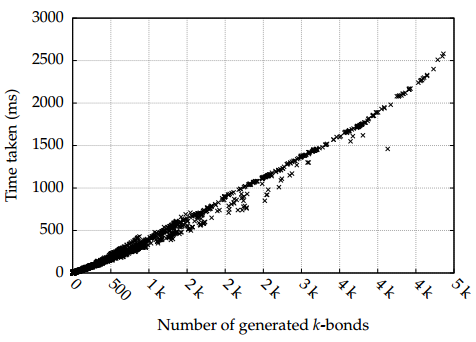
\includegraphics[scale=0.6]{images/capture1_2.PNG}
	\end{figure}

\end{frame}

\begin{frame}
	\frametitle{Evaluace -- kolik řezů algoritmus nezvládne kanonizovat}

\begin{table}[H]
	\caption{Olomoucký kraj -- o kolik více generuje algoritmus ve srovnání se zcela kanonickým [\%]}
	\centering
	\begin{tabular}{c|rrrrrrrr}

\toprule

            &         3 &         4 &         5 &         6 &         7 \\ \midrule
         3  &     0,156 &     0,253 &     0,649 &     1,049 &     1,568 \\
\evenrowcolor
         4  &           &     0,352 &     0,541 &         -  &       -  \\

	\end{tabular}
\end{table}

\end{frame}

\begin{frame}
	\frametitle{Evaluace -- zrychlení kanonickým generováním}

\begin{table}[H]
	\caption{Kolikrát je kanonické generování rychlejší pro dané $k$~(řádky) a~$m$~(sloupce)}
	\centering
	\begin{tabular}{c|rrrrrrrr}

\toprule

   &         2 &         3 &         4 &         5 &         6 &     7 &     8 \\ \midrule
2  &      1.14 &      1.93 &      1.91 &      2.18 &      4.30 &  5.06 &  5.57 \\
\evenrowcolor
3  &      1.97 &      3.47 &      4.49 &      6.69 &      8.31 &     - &     - \\
4  &           &      5.96 &     10.16 &     15.53 &         - &     - &     - \\

	\end{tabular}
\end{table}

\end{frame}

\begin{frame}
	\frametitle{Závěr}

	Cíl práce byl splněn. Algoritmus i~s~implementací (mimo jiné) nejspíše poslouží Centru Dopravního Výzkumu.
\\
\bigskip

Podněty pro další práci: Jak pojmout kanonické generování, aby bylo skutečně kanonické? Jak dále zrychlit implementaci?


\end{frame}


\end{document}
